% XeLaTeX source. Compile: xelatex -interaction=nonstopmode -halt-on-error frontier-proof-audit.tex
% Research note: contains conditional results, not a proof of P=NP.
\documentclass[11pt,a4paper]{article}
\usepackage[margin=19mm,headheight=15pt,footskip=10mm]{geometry}
\usepackage{fontspec}
\setmainfont{Comic Neue}
\setsansfont{Comic Neue}
\setmonofont{Liberation Mono}
\usepackage{amsmath,amssymb,amsthm,mathtools}
\usepackage{xcolor,hyperref,fancyhdr,microtype}
\usepackage{tikz}
\usetikzlibrary{arrows.meta,decorations.pathmorphing}
\definecolor{ink}{HTML}{213B59}
\definecolor{pencil}{HTML}{657784}
\hypersetup{colorlinks=true,urlcolor=ink,linkcolor=ink,pdftitle={P versus NP: Conditional SAT Route and Frontier Width Barrier},pdfauthor={Charalampos Nadiotis}}
\color{ink}
\setlength{\parindent}{0pt}
\setlength{\parskip}{5pt}
\setlength{\emergencystretch}{2em}
\linespread{1.04}
\pagestyle{fancy}
\fancyhf{}
\fancyhead[L]{\footnotesize P\,/\,NP -- formal research audit}
\fancyhead[R]{\footnotesize 2 November 2026}
\fancyfoot[C]{\footnotesize \thepage}
\renewcommand{\headrulewidth}{0.3pt}
\newtheorem{theorem}{Theorem}
\newtheorem{lemma}{Lemma}
\newtheorem{proposition}{Proposition}
\newcommand{\SAT}{\mathsf{SAT}}
\newcommand{\NP}{\mathsf{NP}}
\newcommand{\PP}{\mathsf{P}}
\newcommand{\poly}{\operatorname{poly}}
\begin{document}
\begin{center}
{\LARGE\bfseries P versus NP: What the SAT Frontier Method Proves}\\[2mm]
{\large A conditional reduction, exactness invariant, and exponential-width obstruction}\\[2mm]
Charalampos Nadiotis \quad | \quad PELAOS Tech \quad | \quad 2 November 2026
\end{center}
\vspace{-3mm}
\begin{center}
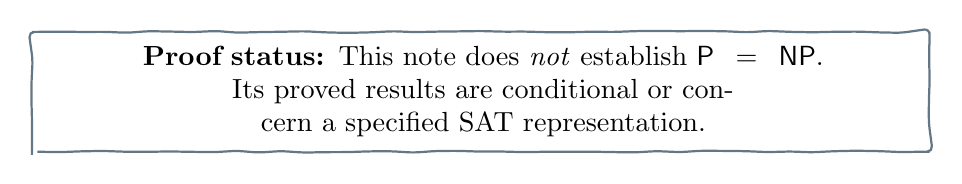
\begin{tikzpicture}
\node[inner sep=5pt,text width=.91\linewidth,align=center] (status) {\textbf{Proof status:} This note does \emph{not} establish $\PP=\NP$.\\ Its proved results are conditional or concern a specified SAT representation.};
\draw[decorate,decoration={random steps,segment length=8pt,amplitude=.35pt},line width=.8pt,color=pencil,rounded corners=2pt]
  (status.south west) -- (status.south east) -- (status.north east) -- (status.north west) -- cycle;
\end{tikzpicture}
\end{center}
\vspace{-3mm}

\section*{1. Exact target}
Let $N=|\langle F\rangle|$ be the bit length of an explicitly encoded Boolean formula $F$. A deterministic algorithm $A$ would resolve the problem in the affirmative if it returned the correct SAT/UNSAT answer \emph{for every formula} and if fixed constants $C,c>0$ existed such that
\[
\boxed{\forall F:\qquad T_A(F)\le C N^c.}
\]
The cost must include representing, constructing, comparing, and updating states, not merely counting nominal transitions.

\begin{theorem}[Conditional route through SAT]
If unrestricted SAT admits a deterministic polynomial-time decision procedure, then $\PP=\NP$.
\end{theorem}
\begin{proof}
By Cook--Levin, every language $L\in\NP$ reduces to SAT by a polynomial-time computable map $r_L$, with $x\in L$ exactly when $r_L(x)$ is satisfiable. If $A$ decides SAT in polynomial time, deciding $L$ consists of computing $r_L(x)$ and then running $A(r_L(x))$. Polynomial bounds compose, so $\NP\subseteq\PP$. The reverse inclusion $\PP\subseteq\NP$ is immediate; hence equality follows.
\end{proof}
This theorem does \emph{not} supply such an $A$. Its assumption is precisely the missing result.

\section*{2. An exact state representation}
Write a CNF as $F=\bigwedge_{j=1}^m C_j$, and fix a variable order $\pi=(v_1,\ldots,v_n)$. After the first $t$ variables, a clause is \emph{active} if it contains both a processed and an unprocessed variable. Let $A_t$ denote the active-clause index set and $w=\max_t|A_t|$.

For a prefix assignment $\alpha$, record the set
\[
S_t(\alpha)=\{j\in A_t:C_j\text{ is already satisfied by }\alpha\}.
\]
Reject $\alpha$ when any clause whose variables have all been processed is false. Merge prefixes with the same active-clause satisfaction set, preserving one witness for each set.

\begin{lemma}[Frontier exactness]
At cut $t$, the stored state set contains exactly the masks $S_t(\alpha)$ reachable from prefixes that satisfy every closed clause. A surviving terminal state exists if and only if $F$ is satisfiable.
\end{lemma}
\begin{proof}
At $t=0$ the empty prefix gives the empty mask unless $F$ contains an empty clause. Suppose the claim holds at cut $t$. For each stored mask, assigning $v_{t+1}$ either truth value updates exactly the clauses newly satisfied by that literal. A clause closing at this step must now be true; otherwise no later assignment could repair it. Dropping a closed clause is safe because it is satisfied and has no unprocessed variable. Untouched clauses need no stored bit. Thus every accepted successor represents a viable extended prefix, and every viable extended prefix arises from one such successor. Two prefixes with the same mask have identical future feasibility: their closed clauses are satisfied, their untouched clauses are unevaluated, and their active clauses have the same already-satisfied pattern. Induction gives the result. At $t=n$ there are no active clauses; survival is equivalent to the existence of a satisfying assignment.
\end{proof}

\section*{3. Complexity: a structural, not universal, bound}
\begin{theorem}[Width-parameterized upper bound]
For a supplied order $\pi$, the exact frontier algorithm admits time and space bounds
\[
T(F,\pi)=\poly(N)\,2^w,\qquad M(F,\pi)=\poly(N)\,2^w.
\]
Consequently, if $w=O(\log N)$, this particular algorithm is polynomial-time on that class of ordered instances.
\end{theorem}
\begin{proof}
At most $2^{|A_t|}\le 2^w$ bitmasks exist at any cut. There are at most $n+1$ cuts and two outgoing truth choices per state. Active-clause metadata, keys, witnesses, bit-mask operations, collision-free state comparisons, and successor generation have polynomial bit cost in the explicitly encoded input size $N$. Multiplying that cost by $O((n+1)2^w)$ gives the claimed bound. If $w\le c\log_2 N$, then $2^w\le N^c$, so the overall bound is polynomial.
\end{proof}
A resource-limited run that terminates with \texttt{limit\_states} or \texttt{limit\_seconds} is \emph{inconclusive}; it is not a SAT or UNSAT certificate.

\section*{4. An exponential obstruction for a fixed order}
\begin{proposition}[Grouped variable order]
Let
\[
F_k=\bigwedge_{i=1}^{k}(x_i\lor y_i),\qquad
\pi=(x_1,\ldots,x_k,y_1,\ldots,y_k).
\]
Immediately after processing all $x_i$, the exact frontier method has $2^k$ distinct reachable masks.
\end{proposition}
\begin{proof}
Each clause crosses this cut, so every clause is active and none is closed. Each assignment $a\in\{0,1\}^k$ to the $x_i$ produces precisely the mask $\{i:a_i=1\}$. Distinct assignments give distinct masks; all are viable because setting every $y_i=1$ satisfies the formula. There are therefore $2^k$ reachable masks.
\end{proof}
The explicit input size is $N=\Theta(k\log(k+1))$ under ordinary binary variable identifiers. Thus $2^k$ grows faster than every fixed polynomial in $N$. The obstruction concerns \emph{this representation and this ordering}. With $(x_1,y_1,\ldots,x_k,y_k)$ instead, the maximum active width is one. This example proves neither a lower bound for every ordering nor $\PP\ne\NP$.

\section*{5. Open proof obligations}
A valid general affirmative proof still requires a fully specified deterministic algorithm for \emph{arbitrary} SAT instances, with (i) unconditional soundness, completeness, and termination and (ii) a worst-case polynomial total bit-cost bound independent of the instance family. For frontier methods, both state growth and the cost of choosing or discovering a useful order must be bounded; finite benchmarks cannot establish those universal quantifiers.

\textbf{Repository evidence:} \href{https://github.com/n0711/P_EQUALS_NP/blob/main/FRONTIER_COMPLEXITY.md}{\texttt{FRONTIER\_COMPLEXITY.md}} documents the invariant, variable-order obstruction, and bounded experiments. \href{https://github.com/n0711/P_EQUALS_NP/blob/main/PROOF_STATUS.md}{\texttt{PROOF\_STATUS.md}} records the proof boundary. Any new claim must be checked against these baselines.\\
\textit{Conclusion: exactness and a width-sensitive bound are established for the specified method; an unconditional proof of $\PP=\NP$ is not.}

\vspace{1mm}
{\footnotesize\textbf{Classical references:} S. A. Cook, \`\`The Complexity of Theorem-Proving Procedures,'' \emph{STOC}, 1971; L. A. Levin, \`\`Universal Search Problems,'' \emph{Problems of Information Transmission}, 1973.}
\end{document}
